\documentclass[tikz]{standalone}

\usepackage{tikz}
\usetikzlibrary{shapes.geometric,calc}

\begin{document}
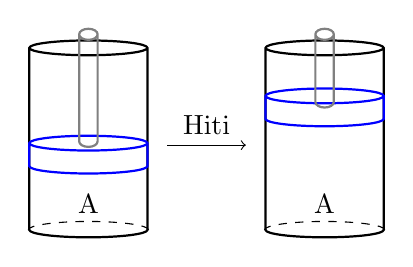
\begin{tikzpicture}
  
  
  \node[cylinder,draw=black,thick,aspect=0.8,
        minimum height=2.5cm,minimum width=1.5cm,
        shape border rotate=90,
        ]
   (A) at (0,0) {};
   
  
  \draw[dashed]
    let \p1 = ($ (A.after bottom) - (A.before bottom) $),
        \n1 = {0.5*veclen(\x1,\y1)},
        \p2 = ($ (A.bottom) - (A.after bottom)!.5!(A.before 			bottom) $),
        \n2 = {veclen(\x2,\y2)}
  in
    (A.before bottom) arc [start angle=0, end angle=180,
    x radius=\n1, y radius=\n2];
    
 \node[] at (0,-0.75) {A};
    
     \node[cylinder,draw=blue,thick,aspect=0.8,
        minimum height=0.4cm,minimum width=1.5cm,
        shape border rotate=90,
        ]
   (B) at (0,-0.2) {};
   
    
     \node[cylinder,draw=gray,thick,aspect=0.6,
        minimum height=1.5cm,minimum width=0.2cm,
        shape border rotate=90,
        ]
   (F) at (0,0.65) {};
   
%--------------------
   
 \node[cylinder,draw=black,thick,aspect=0.8,
        minimum height=2.5cm,minimum width=1.5cm,
        shape border rotate=90,
        ]
   (C) at (3,0) {};
   
  
  \draw[dashed]
    let \p1 = ($ (C.after bottom) - (C.before bottom) $),
        \n1 = {0.5*veclen(\x1,\y1)},
        \p2 = ($ (C.bottom) - (C.after bottom)!.5!(C.before 			bottom) $),
        \n2 = {veclen(\x2,\y2)}
  in
    (C.before bottom) arc [start angle=0, end angle=180,
    x radius=\n1, y radius=\n2];
    
 \node[] at (3,-0.75) {A};
    
   
\draw[->] (1,0) -- (2,0) ;

\node [] at (1.5,0.25) {Hiti};
 
 
 \node[cylinder,draw=blue,thick,aspect=0.8,
        minimum height=0.4cm,minimum width=1.5cm,
        shape border rotate=90,
        ]
   (G) at (3,0.4) {};
   
    
     \node[cylinder,draw=gray,thick,aspect=0.6,
        minimum height=1cm,minimum width=0.2cm,
        shape border rotate=90,
        ]
   (H) at (3,0.9) {}; 
 
\end{tikzpicture}
\end{document}